% Options for packages loaded elsewhere
\PassOptionsToPackage{unicode}{hyperref}
\PassOptionsToPackage{hyphens}{url}
%
\documentclass[
]{article}
\usepackage{lmodern}
\usepackage{amssymb,amsmath}
\usepackage{ifxetex,ifluatex}
\ifnum 0\ifxetex 1\fi\ifluatex 1\fi=0 % if pdftex
  \usepackage[T1]{fontenc}
  \usepackage[utf8]{inputenc}
  \usepackage{textcomp} % provide euro and other symbols
\else % if luatex or xetex
  \usepackage{unicode-math}
  \defaultfontfeatures{Scale=MatchLowercase}
  \defaultfontfeatures[\rmfamily]{Ligatures=TeX,Scale=1}
\fi
% Use upquote if available, for straight quotes in verbatim environments
\IfFileExists{upquote.sty}{\usepackage{upquote}}{}
\IfFileExists{microtype.sty}{% use microtype if available
  \usepackage[]{microtype}
  \UseMicrotypeSet[protrusion]{basicmath} % disable protrusion for tt fonts
}{}
\makeatletter
\@ifundefined{KOMAClassName}{% if non-KOMA class
  \IfFileExists{parskip.sty}{%
    \usepackage{parskip}
  }{% else
    \setlength{\parindent}{0pt}
    \setlength{\parskip}{6pt plus 2pt minus 1pt}}
}{% if KOMA class
  \KOMAoptions{parskip=half}}
\makeatother
\usepackage{xcolor}
\IfFileExists{xurl.sty}{\usepackage{xurl}}{} % add URL line breaks if available
\IfFileExists{bookmark.sty}{\usepackage{bookmark}}{\usepackage{hyperref}}
\hypersetup{
  pdftitle={Flujo de análisis en clasificación supervisada},
  pdfauthor={Laura Rodríguez Navas},
  hidelinks,
  pdfcreator={LaTeX via pandoc}}
\urlstyle{same} % disable monospaced font for URLs
\usepackage[margin=1in]{geometry}
\usepackage{color}
\usepackage{fancyvrb}
\newcommand{\VerbBar}{|}
\newcommand{\VERB}{\Verb[commandchars=\\\{\}]}
\DefineVerbatimEnvironment{Highlighting}{Verbatim}{commandchars=\\\{\}}
% Add ',fontsize=\small' for more characters per line
\usepackage{framed}
\definecolor{shadecolor}{RGB}{248,248,248}
\newenvironment{Shaded}{\begin{snugshade}}{\end{snugshade}}
\newcommand{\AlertTok}[1]{\textcolor[rgb]{0.94,0.16,0.16}{#1}}
\newcommand{\AnnotationTok}[1]{\textcolor[rgb]{0.56,0.35,0.01}{\textbf{\textit{#1}}}}
\newcommand{\AttributeTok}[1]{\textcolor[rgb]{0.77,0.63,0.00}{#1}}
\newcommand{\BaseNTok}[1]{\textcolor[rgb]{0.00,0.00,0.81}{#1}}
\newcommand{\BuiltInTok}[1]{#1}
\newcommand{\CharTok}[1]{\textcolor[rgb]{0.31,0.60,0.02}{#1}}
\newcommand{\CommentTok}[1]{\textcolor[rgb]{0.56,0.35,0.01}{\textit{#1}}}
\newcommand{\CommentVarTok}[1]{\textcolor[rgb]{0.56,0.35,0.01}{\textbf{\textit{#1}}}}
\newcommand{\ConstantTok}[1]{\textcolor[rgb]{0.00,0.00,0.00}{#1}}
\newcommand{\ControlFlowTok}[1]{\textcolor[rgb]{0.13,0.29,0.53}{\textbf{#1}}}
\newcommand{\DataTypeTok}[1]{\textcolor[rgb]{0.13,0.29,0.53}{#1}}
\newcommand{\DecValTok}[1]{\textcolor[rgb]{0.00,0.00,0.81}{#1}}
\newcommand{\DocumentationTok}[1]{\textcolor[rgb]{0.56,0.35,0.01}{\textbf{\textit{#1}}}}
\newcommand{\ErrorTok}[1]{\textcolor[rgb]{0.64,0.00,0.00}{\textbf{#1}}}
\newcommand{\ExtensionTok}[1]{#1}
\newcommand{\FloatTok}[1]{\textcolor[rgb]{0.00,0.00,0.81}{#1}}
\newcommand{\FunctionTok}[1]{\textcolor[rgb]{0.00,0.00,0.00}{#1}}
\newcommand{\ImportTok}[1]{#1}
\newcommand{\InformationTok}[1]{\textcolor[rgb]{0.56,0.35,0.01}{\textbf{\textit{#1}}}}
\newcommand{\KeywordTok}[1]{\textcolor[rgb]{0.13,0.29,0.53}{\textbf{#1}}}
\newcommand{\NormalTok}[1]{#1}
\newcommand{\OperatorTok}[1]{\textcolor[rgb]{0.81,0.36,0.00}{\textbf{#1}}}
\newcommand{\OtherTok}[1]{\textcolor[rgb]{0.56,0.35,0.01}{#1}}
\newcommand{\PreprocessorTok}[1]{\textcolor[rgb]{0.56,0.35,0.01}{\textit{#1}}}
\newcommand{\RegionMarkerTok}[1]{#1}
\newcommand{\SpecialCharTok}[1]{\textcolor[rgb]{0.00,0.00,0.00}{#1}}
\newcommand{\SpecialStringTok}[1]{\textcolor[rgb]{0.31,0.60,0.02}{#1}}
\newcommand{\StringTok}[1]{\textcolor[rgb]{0.31,0.60,0.02}{#1}}
\newcommand{\VariableTok}[1]{\textcolor[rgb]{0.00,0.00,0.00}{#1}}
\newcommand{\VerbatimStringTok}[1]{\textcolor[rgb]{0.31,0.60,0.02}{#1}}
\newcommand{\WarningTok}[1]{\textcolor[rgb]{0.56,0.35,0.01}{\textbf{\textit{#1}}}}
\usepackage{graphicx,grffile}
\makeatletter
\def\maxwidth{\ifdim\Gin@nat@width>\linewidth\linewidth\else\Gin@nat@width\fi}
\def\maxheight{\ifdim\Gin@nat@height>\textheight\textheight\else\Gin@nat@height\fi}
\makeatother
% Scale images if necessary, so that they will not overflow the page
% margins by default, and it is still possible to overwrite the defaults
% using explicit options in \includegraphics[width, height, ...]{}
\setkeys{Gin}{width=\maxwidth,height=\maxheight,keepaspectratio}
% Set default figure placement to htbp
\makeatletter
\def\fps@figure{htbp}
\makeatother
\setlength{\emergencystretch}{3em} % prevent overfull lines
\providecommand{\tightlist}{%
  \setlength{\itemsep}{0pt}\setlength{\parskip}{0pt}}
\setcounter{secnumdepth}{5}

\title{Flujo de análisis en clasificación supervisada}
\usepackage{etoolbox}
\makeatletter
\providecommand{\subtitle}[1]{% add subtitle to \maketitle
  \apptocmd{\@title}{\par {\large #1 \par}}{}{}
}
\makeatother
\subtitle{Métodos supervisados}
\author{Laura Rodríguez Navas}
\date{Septiembre 2020}

\begin{document}
\maketitle

{
\setcounter{tocdepth}{2}
\tableofcontents
}
Comenzamos cargando los paquetes necesarios.

\begin{Shaded}
\begin{Highlighting}[]
\KeywordTok{library}\NormalTok{(caret)}
\KeywordTok{library}\NormalTok{(dplyr)}
\KeywordTok{library}\NormalTok{(doParallel)}
\end{Highlighting}
\end{Shaded}

\hypertarget{descripciuxf3n}{%
\subsection{Descripción}\label{descripciuxf3n}}

Para la realización del ejercicio propuesto se ha elegido la competición
en Kaggle: \textbf{Real or Not? NLP with Disaster Tweets}. El dataset de
la competición se puede encontrar en el siguiente enlace:
\url{https://www.kaggle.com/c/nlp-getting-started/data}. Este dataset,
con 10.876 instancias, contiene 4 variables explicativas: \textbf{id},
\textbf{keyword}, \textbf{location} y \textbf{text}, y dos valores en la
variable clase \textbf{target} (0 y 1). La variable clase es binaria,
así que, vamos a aprender un modelo de clasificación binaria. El
objetivo de este modelo será predecir si dado un tweet, este tweet trata
sobre un desastre real o no. Si un tweet trata sobre un desastre real,
se predice un 1. Si no, se predice un 0.

La métrica de evaluación esperada por la competición es
\href{https://www.kaggle.com/c/nlp-getting-started/overview/evaluation}{F1}.
Y se calcula de la siguiente manera:

\begin{center}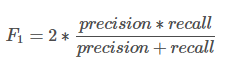
\includegraphics[width=0.3\linewidth]{F1_score} \end{center}

donde:

\begin{center}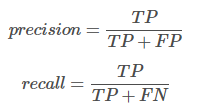
\includegraphics[width=0.25\linewidth]{F1_score_2} \end{center}

La partición inicial train-test, no se tiene que realizar, ya que las
instancias de train y test ya vienen definidas en el dataset de la
competición (ficheros \textbf{train.csv} y \textbf{test.csv}).

A continuación, cargaremos el conjunto de datos de train y test,
nombrando los valores perdidos como \textbf{NA} para que los podamos
tratar más adelante, y mostraremos sus dimensiones.

\begin{Shaded}
\begin{Highlighting}[]
\NormalTok{train <-}\StringTok{ }\KeywordTok{read.csv}\NormalTok{(}\StringTok{"train.csv"}\NormalTok{, }\DataTypeTok{na.strings=}\KeywordTok{c}\NormalTok{(}\StringTok{""}\NormalTok{, }\StringTok{"NA"}\NormalTok{))}
\NormalTok{test <-}\StringTok{ }\KeywordTok{read.csv}\NormalTok{(}\StringTok{"test.csv"}\NormalTok{, }\DataTypeTok{na.strings=}\KeywordTok{c}\NormalTok{(}\StringTok{""}\NormalTok{, }\StringTok{"NA"}\NormalTok{))}
\KeywordTok{dim}\NormalTok{(train)}
\end{Highlighting}
\end{Shaded}

\begin{verbatim}
## [1] 7613    5
\end{verbatim}

\begin{Shaded}
\begin{Highlighting}[]
\KeywordTok{dim}\NormalTok{(test)}
\end{Highlighting}
\end{Shaded}

\begin{verbatim}
## [1] 3263    4
\end{verbatim}

El conjunto de datos de train contiene 7613 instancias y el conjunto de
datos de test contiene 3263 instancias. Cada instancia de estos
conjuntos contiene la siguiente información:

\begin{itemize}
\tightlist
\item
  \textbf{id}: un identificador único para cada tweet.
\item
  \textbf{keyword}: una palabra clave del tweet.
\item
  \textbf{location}: la ubicación desde la que se envió el tweet.
\item
  \textbf{text}: el texto del tweet.
\item
  \textbf{target}: solo en el conjunto de datos de train porqué es la
  variable clase a predecir. Indica si un tweet es sobre un desastre
  real (1) o no (0).
\end{itemize}

\begin{Shaded}
\begin{Highlighting}[]
\KeywordTok{str}\NormalTok{(train, }\DataTypeTok{width =} \DecValTok{85}\NormalTok{, }\DataTypeTok{strict.width =} \StringTok{"cut"}\NormalTok{)}
\end{Highlighting}
\end{Shaded}

\begin{verbatim}
## 'data.frame':    7613 obs. of  5 variables:
##  $ id      : int  1 4 5 6 7 8 10 13 14 15 ...
##  $ keyword : chr  NA NA NA NA ...
##  $ location: chr  NA NA NA NA ...
##  $ text    : chr  "Our Deeds are the Reason of this #earthquake May ALLAH Forgive "..
##  $ target  : int  1 1 1 1 1 1 1 1 1 1 ...
\end{verbatim}

\begin{Shaded}
\begin{Highlighting}[]
\KeywordTok{str}\NormalTok{(test, }\DataTypeTok{width =} \DecValTok{85}\NormalTok{, }\DataTypeTok{strict.width =} \StringTok{"cut"}\NormalTok{)}
\end{Highlighting}
\end{Shaded}

\begin{verbatim}
## 'data.frame':    3263 obs. of  4 variables:
##  $ id      : int  0 2 3 9 11 12 21 22 27 29 ...
##  $ keyword : chr  NA NA NA NA ...
##  $ location: chr  NA NA NA NA ...
##  $ text    : chr  "Just happened a terrible car crash" "Heard about #earthquake is"..
\end{verbatim}

Unimos los conjuntos de train y test (\emph{7613 + 3263 observaciones})
para poder analizar y extraer los sentimientos más adelante.

\begin{Shaded}
\begin{Highlighting}[]
\NormalTok{complete_df <-}\StringTok{ }\KeywordTok{bind_rows}\NormalTok{(train, test)}
\KeywordTok{dim}\NormalTok{(complete_df)}
\end{Highlighting}
\end{Shaded}

\begin{verbatim}
## [1] 10876     5
\end{verbatim}

El análisis de sentimientos es una técnica de \emph{Machine Learning},
basada en el
\href{https://www.kdnuggets.com/2017/02/natural-language-processing-key-terms-explained.html}{procesado
del lenguaje natural}, que pretende obtener información subjetiva de una
serie de textos. Su aplicación es este caso, consiste en resolver si un
tweet es real o no real en relación a un desastre.

Echamos un vistazo más de cerca a las variables del nuevo conjunto de
datos \textbf{complete\_df}.

\begin{Shaded}
\begin{Highlighting}[]
\KeywordTok{summary}\NormalTok{(complete_df)}
\end{Highlighting}
\end{Shaded}

\begin{verbatim}
##        id          keyword            location             text          
##  Min.   :    0   Length:10876       Length:10876       Length:10876      
##  1st Qu.: 2719   Class :character   Class :character   Class :character  
##  Median : 5438   Mode  :character   Mode  :character   Mode  :character  
##  Mean   : 5438                                                           
##  3rd Qu.: 8156                                                           
##  Max.   :10875                                                           
##                                                                          
##      target    
##  Min.   :0.00  
##  1st Qu.:0.00  
##  Median :0.00  
##  Mean   :0.43  
##  3rd Qu.:1.00  
##  Max.   :1.00  
##  NA's   :3263
\end{verbatim}

Vemos que la variable \textbf{id} es solo un identificador único y la
eliminaremos.

\begin{Shaded}
\begin{Highlighting}[]
\NormalTok{complete_df}\OperatorTok{$}\NormalTok{id <-}\StringTok{ }\OtherTok{NULL}
\KeywordTok{dim}\NormalTok{(complete_df)}
\end{Highlighting}
\end{Shaded}

\begin{verbatim}
## [1] 10876     4
\end{verbatim}

\begin{itemize}
\tightlist
\item
  Confirmamos que la variable \textbf{target} es la variable
  dependiente, la que nos interesa es predecir. Al observarla podemos
  decir que el 32\% de los tweets en realidad se refieren a un desastre
  y el 43\% no.
\end{itemize}

\hypertarget{gruxe1ficas-de-visualizaciuxf3n}{%
\subsection{Gráficas de
visualización}\label{gruxe1ficas-de-visualizaciuxf3n}}

Relacionado con la descripción anterior, mostraremos algunas gráficas de
visualización de algunas variables de interés. Pero primero tenemos que
categorizar la variable a predecir, ya que inicialmente es de tipo
entero.

\begin{Shaded}
\begin{Highlighting}[]
\NormalTok{complete_df}\OperatorTok{$}\NormalTok{target <-}\StringTok{ }\KeywordTok{as.factor}\NormalTok{(}\KeywordTok{ifelse}\NormalTok{(complete_df}\OperatorTok{$}\NormalTok{target }\OperatorTok{==}\StringTok{ }\DecValTok{0}\NormalTok{, }\StringTok{"No"}\NormalTok{, }\StringTok{"Yes"}\NormalTok{))}
\KeywordTok{str}\NormalTok{(complete_df, }\DataTypeTok{width =} \DecValTok{85}\NormalTok{, }\DataTypeTok{strict.width =} \StringTok{"cut"}\NormalTok{)}
\end{Highlighting}
\end{Shaded}

\begin{verbatim}
## 'data.frame':    10876 obs. of  4 variables:
##  $ keyword : chr  NA NA NA NA ...
##  $ location: chr  NA NA NA NA ...
##  $ text    : chr  "Our Deeds are the Reason of this #earthquake May ALLAH Forgive "..
##  $ target  : Factor w/ 2 levels "No","Yes": 2 2 2 2 2 2 2 2 2 2 ...
\end{verbatim}

La primera visualización representa la distribución de la variable a
predecir.

\begin{Shaded}
\begin{Highlighting}[]
\KeywordTok{ggplot}\NormalTok{(train, }\KeywordTok{aes}\NormalTok{(}\DataTypeTok{x=}\NormalTok{target)) }\OperatorTok{+}\StringTok{ }\KeywordTok{geom_bar}\NormalTok{(}\KeywordTok{aes}\NormalTok{(}\DataTypeTok{fill=}\NormalTok{target))}
\end{Highlighting}
\end{Shaded}

\begin{center}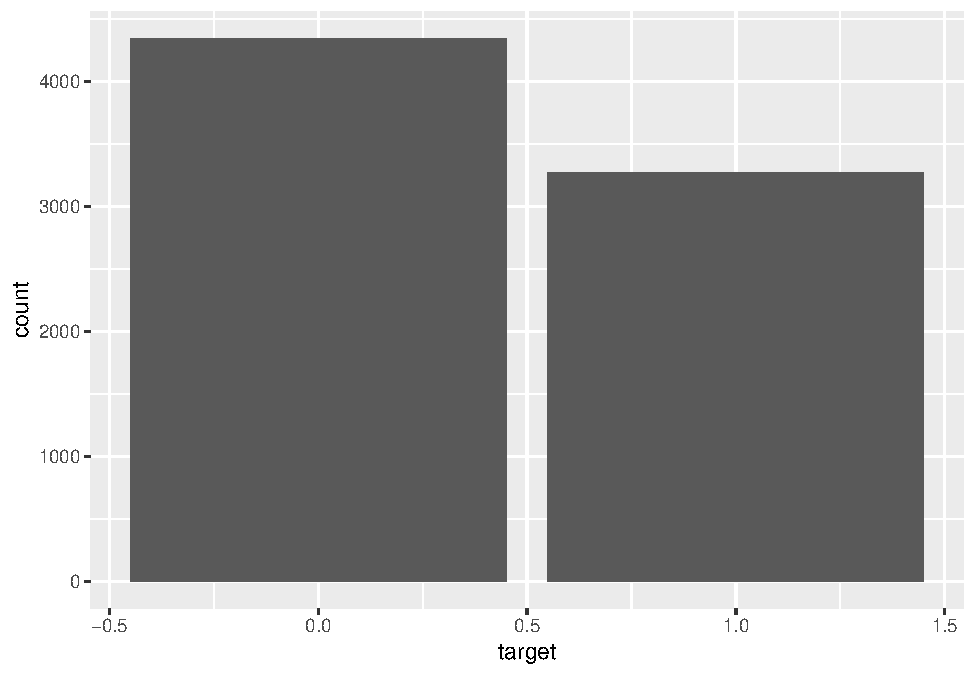
\includegraphics[width=0.7\linewidth]{document_files/figure-latex/unnamed-chunk-10-1} \end{center}

\end{document}
